\documentclass[tikz,border=8pt]{standalone}
\usepackage{tikz}
\usetikzlibrary{shapes,arrows,positioning}
\tikzstyle{proc}=[rectangle,draw,rounded corners,fill=blue!10,align=center,minimum width=3.4cm,minimum height=0.9cm,font=\small]
\tikzstyle{dec}=[diamond,draw,fill=green!10,align=center,aspect=2,font=\small]
\tikzstyle{term}=[rectangle,draw,rounded corners=8pt,fill=gray!15,align=center,minimum width=2.6cm,minimum height=0.9cm,font=\small\bfseries]
\tikzstyle{arr}=[->,thick]
\begin{document}
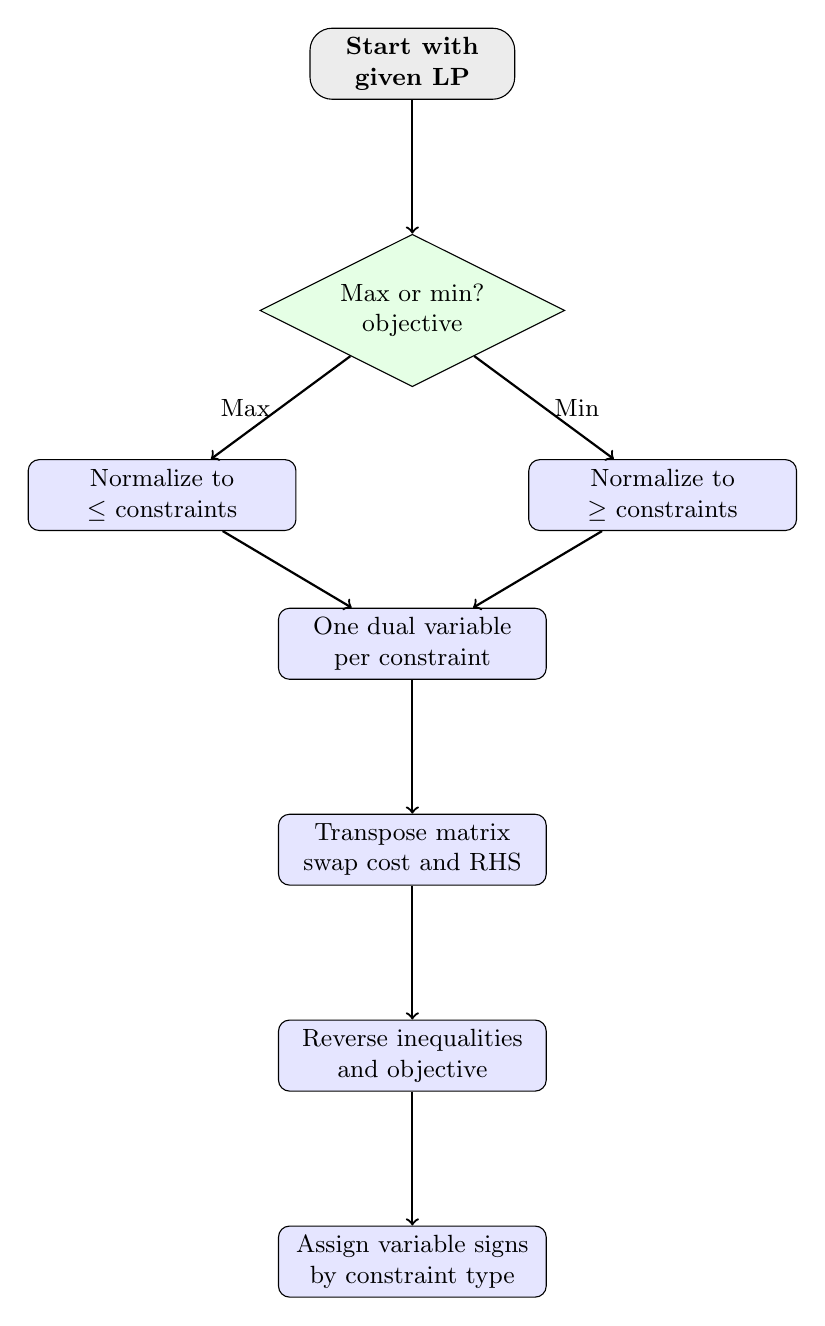
\begin{tikzpicture}[node distance=1.7cm]
\node (A) [term] {Start with\\given LP};
\node (B) [dec, below=of A] {Max or min?\\objective};
\node (C) [proc, below left=1.4cm and 0.5cm of B] {Normalize to\\$\leq$ constraints};
\node (D) [proc, below right=1.4cm and 0.5cm of B] {Normalize to\\$\geq$ constraints};
\node (E) [proc, below=2.8cm of B] {One dual variable\\per constraint};
\node (F) [proc, below=of E] {Transpose matrix\\swap cost and RHS};
\node (G) [proc, below=of F] {Reverse inequalities\\and objective};
\node (H) [proc, below=of G] {Assign variable signs\\by constraint type};
\draw [arr] (A) -- (B);
\draw [arr] (B) -- node [left, font=\small] {Max} (C);
\draw [arr] (B) -- node [right, font=\small] {Min} (D);
\draw [arr] (C) -- (E);
\draw [arr] (D) -- (E);
\draw [arr] (E) -- (F);
\draw [arr] (F) -- (G);
\draw [arr] (G) -- (H);
\end{tikzpicture}
\end{document}
